\documentclass[11pt]{article}
\usepackage{float}
%
%Margin - 1 inch on all sides
%
\usepackage[letterpaper]{geometry}
\usepackage{times}
\usepackage{amsmath}
\geometry{top=0.75in, bottom=0.75in, left=0.75in, right=0.75in}

\pagenumbering{gobble}

\usepackage{ragged2e}
\usepackage{mwe}

\usepackage{multicol}

\usepackage{tabularx}

\setlength{\RaggedRightParfillskip}{.25\textwidth plus 1fil}
\setlength{\RaggedRightRightskip}{0pt plus .1\textwidth}
\setlength{\RaggedRightParindent}{1em}


\usepackage{listings}
\usepackage{color}

\definecolor{dkgreen}{rgb}{0,0.6,0}
\definecolor{gray}{rgb}{0.5,0.5,0.5}
\definecolor{mauve}{rgb}{0.58,0,0.82}
\lstset{frame=tb,
    language=[x86masm]assembler,
    aboveskip=3mm,
    belowskip=3mm,
    showstringspaces=false,
    columns=flexible,
    basicstyle={\small\ttfamily},
    numbers=none,
    numberstyle=\tiny\color{gray},
    keywordstyle=\color{blue},
    commentstyle=\color{dkgreen},
    stringstyle=\color{mauve},
    breaklines=true,
    breakatwhitespace=true,
    tabsize=3
}

\graphicspath{{../}}

\title{CSCE 451 March 27 Lab}
\author{Benton Guess\{bguess10@tamu.edu\}}
\date{March 27, 2020}

\begin{document}
\maketitle

\section*{Challenge 1}
\subsection*{Goal}
Get it to print the "you did it" string

\subsection*{Steps}
I begin by looking for the string referenced in assignment after processing it with \texttt{radare2}. To process it, i begen by running a \texttt{aaa}, which disassembles and analyzes using reasonable settings (nothing too crazy). Then I ran a \texttt{s main}, which able to seek and find the main entry point. Radare labels strings with the text they feature, so I just looked for a string constant that was similar to the "you did it" text. It was listed here in this segment of control flow. We confirm this in the rodata

\begin{lstlisting}
    0x080486a1      cmp dword [var_94h], 2
    0x080486a8      jne 0x80486c1
    0x080486aa      sub esp, 0xc
    0x080486ad      push str.You_did_it ; 0x8048788 ; const char *s
    0x080486b2      call puts          ; sym.imp.puts ; int puts(const char *s)
    ...
    ;-- str.You_did_it:
    0x08048788          .string "You did it!" ; len=12
\end{lstlisting}
From here I could immediately discover that condition we desired was to increment this stack label by 2. I was able to identify to places in the assembly where this happens. Here I used the \texttt{r2dec} tool, somewhat of a midway between a decompiler and disassembler, which preserves our register operations, but reduces the control flow to the language statements. From here I identified two places where this is incremented.

\lstset{frame=tb,
    language=c,
    aboveskip=3mm,
    belowskip=3mm,
    showstringspaces=false,
    columns=flexible,
    basicstyle={\small\ttfamily},
    numbers=none,
    numberstyle=\tiny\color{gray},
    keywordstyle=\color{blue},
    commentstyle=\color{dkgreen},
    stringstyle=\color{mauve},
    breaklines=true,
    breakatwhitespace=true,
    tabsize=3
}
\begin{lstlisting}
    eax = f1 (0xc);
    if (eax == var_98h) {
        printf (format);
        eax = s2;
        eax += 4;
        eax = *(eax);
        eax = strncmp (format, eax, 0x14);
        if (eax != 0) {
            goto label_1;
        }
        var_94h++;
    } else {
        eax = f2 (0xd);
        if (eax != var_98h) {
            goto label_1;
        }
        printf (format);
        eax = s2;
        eax += 8;
        eax = *(eax);
        eax = strncmp (format, eax, 0xc);
        if (eax != 0) {
            goto label_1;
        }
        var_94h++;
    }
\end{lstlisting}

We see there is two places where this happens, and we can see that there are two functions, f1 and f2, being used to compare constants to var\_98h. I then seeked those two functions in radare2

\lstset{frame=tb,
    language=[x86masm]assembler,
    aboveskip=3mm,
    belowskip=3mm,
    showstringspaces=false,
    columns=flexible,
    basicstyle={\small\ttfamily},
    numbers=none,
    numberstyle=\tiny\color{gray},
    keywordstyle=\color{blue},
    commentstyle=\color{dkgreen},
    stringstyle=\color{mauve},
    breaklines=true,
    breakatwhitespace=true,
    tabsize=3
}

\begin{lstlisting}
    11: sym.f1 (int32_t arg_8h);
    ; arg int32_t arg_8h @ ebp+0x8
    0x0804853b      push ebp
    0x0804853c      mov ebp, esp
    0x0804853e      mov eax, dword [arg_8h]
    0x08048541      add eax, 5
    0x08048544      pop ebp
    0x08048545      ret
    11: sym.f2 (int32_t arg_8h);
    ; arg int32_t arg_8h @ ebp+0x8
    0x08048546      push ebp
    0x08048547      mov ebp, esp
    0x08048549      mov eax, dword [arg_8h]
    0x0804854c      add eax, 3
    0x0804854f      pop ebp
    0x08048550      ret
\end{lstlisting}

We can see that f1 adds 5 to an argument and returns with f2 adding 3. This makes our first condition only work when our 98h is equal to $12 + 5 = 17$ and our second condition is $13 + 3 = 16$. From here i investigated what our strcmp is actually comparing, which comes from an fgets on a file called "strings". This is done over a loop, so I assume from this that the two strings I am looking for are going to be the 17th and the 16th in a file called strings. Also, from here I can see that the code is being compared to that s2 string, which comes from the argv of the main function. I found the 17th and 16th strings, then used them as the arguments and got this as the result.

\subsection*{Goal}
\begin{lstlisting}
    [bentonguess@benton-pc march_27_lab_test]$ ./re_challenege1 deregister_tm_clones __JCR_LIST__
    __JCR_LIST__
    deregister_tm_clones
    You did it!
\end{lstlisting}


\subsection*{CFD}
\begin{figure}[H]
    \centering
    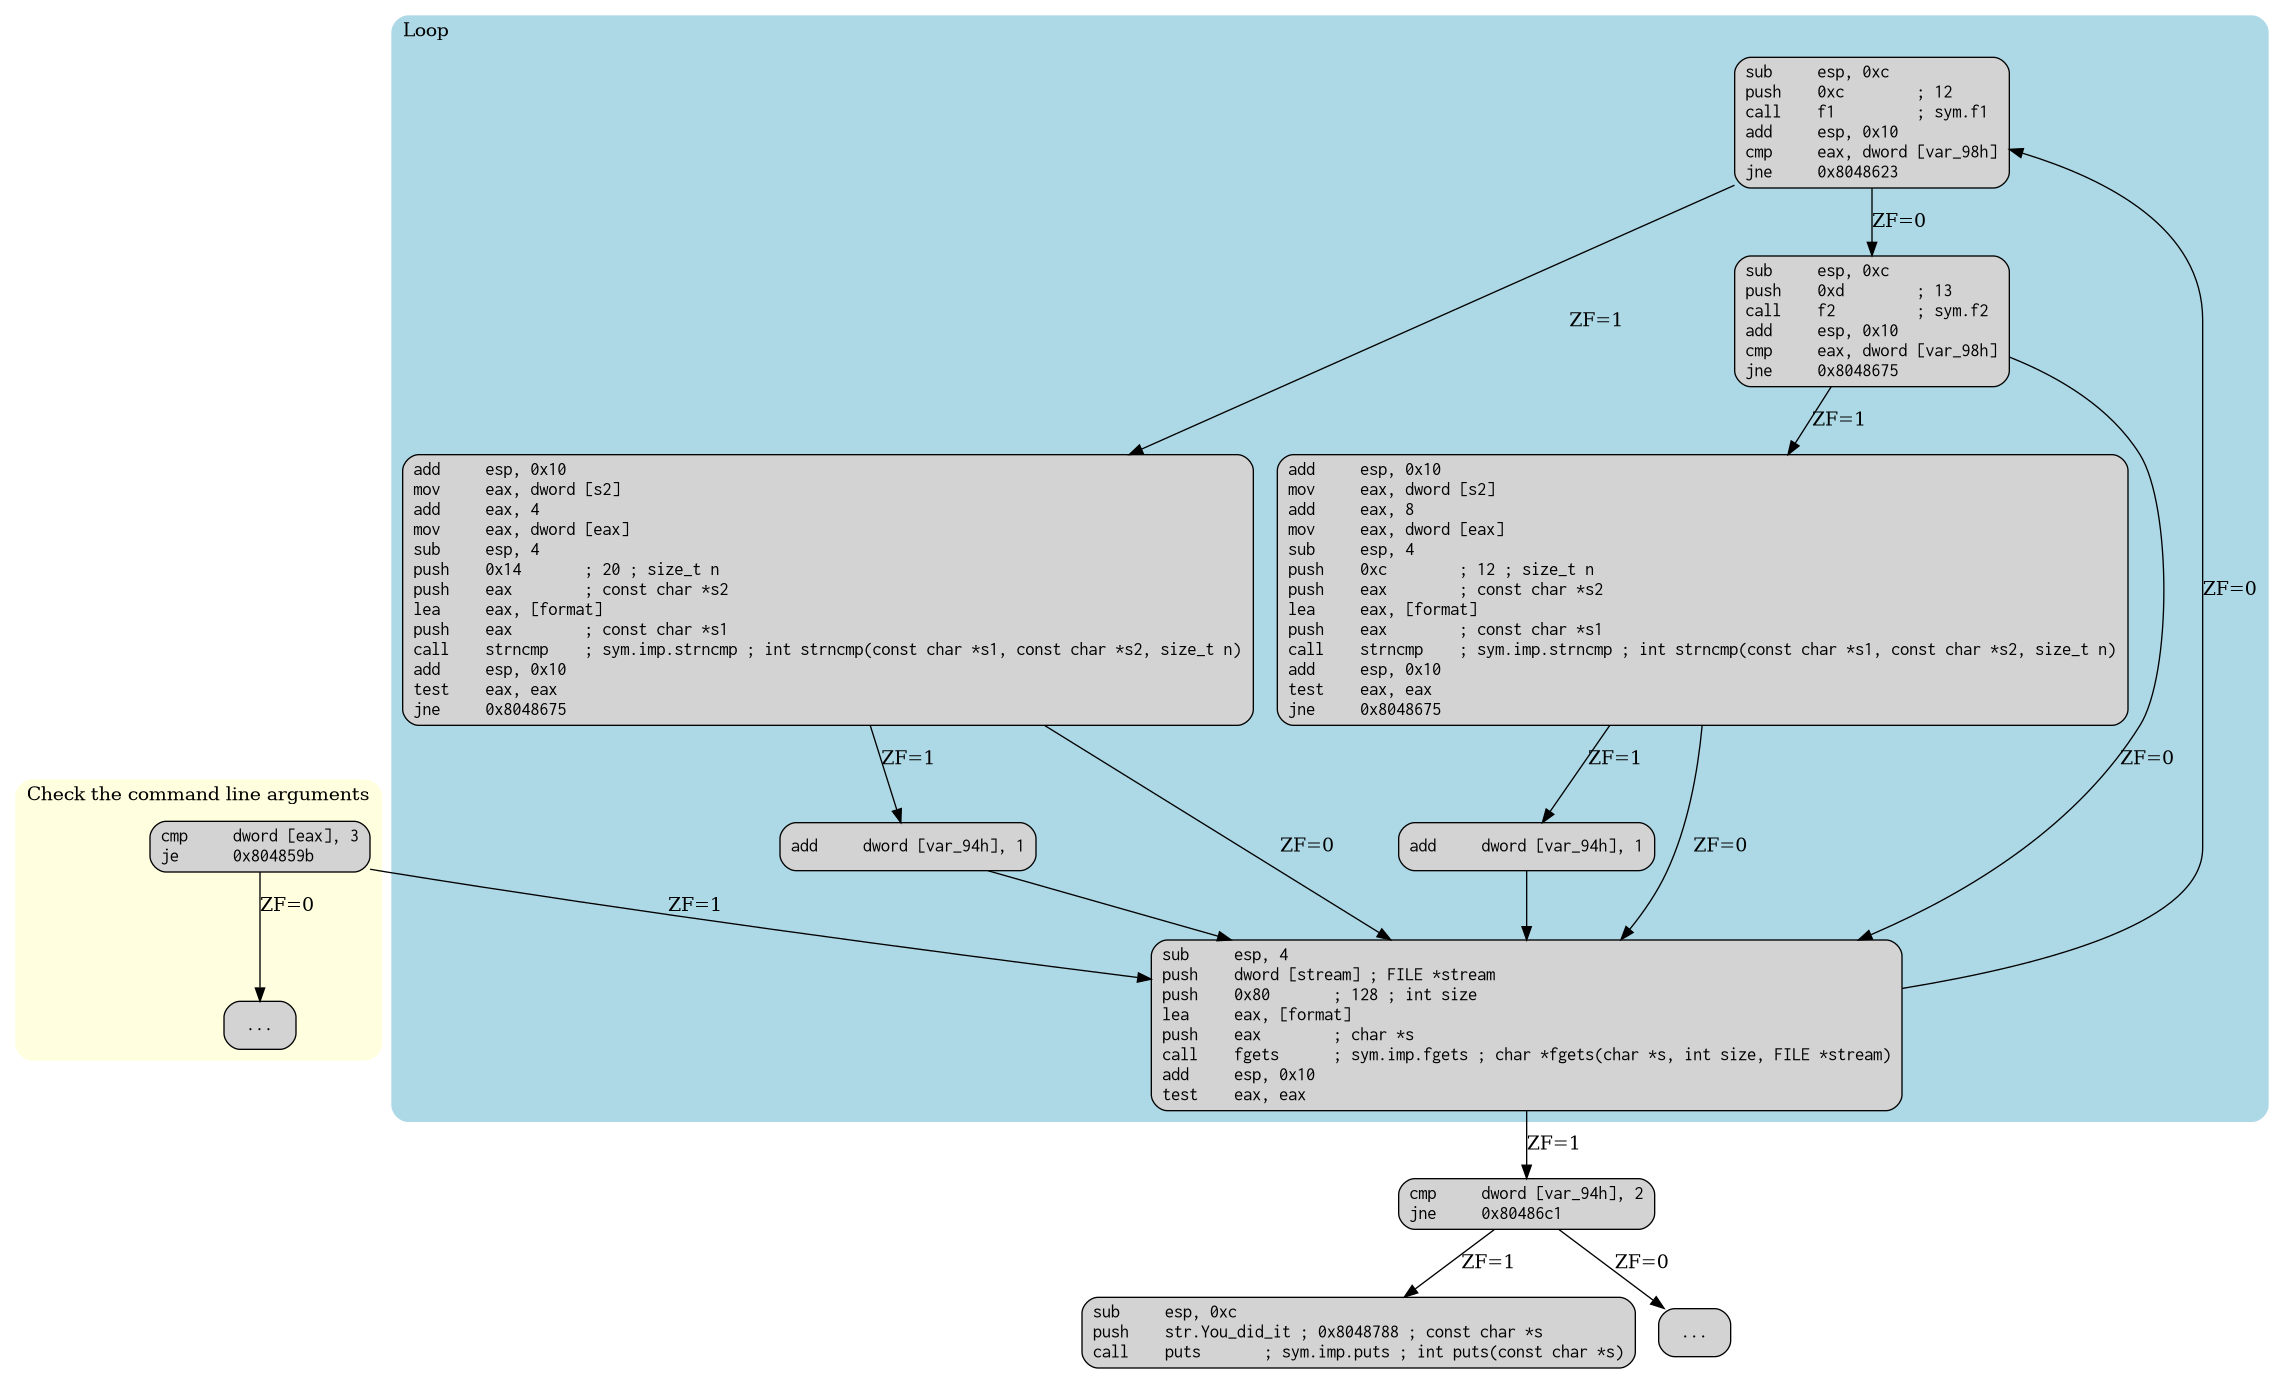
\includegraphics[width=0.99\linewidth]{./graphviz/challenge1.png}
\end{figure}


\section*{Challenge 2}
\subsection*{Goal}
Get the "you are great at this" string to print.
\subsection*{Steps}
After analyzing this the same way as the previous problem and looking at the disassembly, this looked quite strange in terms of the number of variables. It seems like either there was some strange optimizations performed, or that a stack array is being missed by the disassembler. Regardless, looking at the decompiled code is not very helpful with the strange stack we are given.

This looks to be a password search based on the strings saying stuff like "enter your password", there are also 3 calls to \texttt{strtok}, a few calls to \texttt{puts()}, then the program does a string compare on the variable that the last 2 strtoks edited, in the following code you can see this:

\begin{lstlisting}
0x08048816      push    0x8048999  ; const char *s2
0x0804881b      lea     eax, [s1]
0x08048821      push    eax        ; char *s1
0x08048822      call    strtok     ; sym.imp.strtok ; char *strtok(char *s1, const char *s2)
0x08048827      add     esp, 0x10
0x0804882a      mov     dword [s2], eax
0x08048830      sub     esp, 8
0x08048833      push    0x804899b  ; const char *s2
0x08048838      push    0          ; char *s1
0x0804883a      call    strtok     ; sym.imp.strtok ; char *strtok(char *s1, const char *s2)
0x0804883f      add     esp, 0x10
0x08048842      mov     dword [s2], eax
0x08048848      sub     esp, 0xc
0x0804884b      push    dword [s2] ; const char *s
0x08048851      call    puts       ; sym.imp.puts ; int puts(const char *s)
0x08048856      add     esp, 0x10
0x08048859      sub     esp, 8
0x0804885c      push    0x804899d  ; const char *s2
0x08048861      push    dword [s2] ; char *s1
0x08048867      call    strtok     ; sym.imp.strtok ; char *strtok(char *s1, const char *s2)
0x0804886c      add     esp, 0x10
0x0804886f      mov     dword [s2], eax
0x08048875      sub     esp, 0xc
0x08048878      push    dword [s2] ; const char *s
0x0804887e      call    puts       ; sym.imp.puts ; int puts(const char *s)
0x08048883      add     esp, 0x10
0x08048886      sub     esp, 4
0x08048889      push    8          ; 8 ; size_t n
0x0804888b      push    dword [s2] ; const char *s2
0x08048891      lea     eax, [s]
0x08048894      push    eax        ; const char *s1
0x08048895      call    strncmp    ; sym.imp.strncmp ; int strncmp(const char *s1, const char *s2, size_t n)
0x0804889a      add     esp, 0x10
\end{lstlisting}

Since there was plenty of stuff going in with string tokenization and a very messy stack, I felt that GDB was the best way to do this. I set the password to "benton" and broke at the strcmp function. Then I had gathered the locations of the two strings from this section of code produced by radare.
\begin{lstlisting}
    ; var int32_t var_4h @ ebp-0x4
    ; var char *s2 @ ebp-0x178
    ; var char *s @ ebp-0x70
\end{lstlisting}

\begin{lstlisting}
    Breakpoint 1, 0x08048895 in main ()
    (gdb) print (char*)($ebp-0x70)
    $1 = 0xffffd598 "benton"
    (gdb) print *(char**)($ebp-0x70)
    $2 = 0x746e6562 <error: Cannot access memory at address 0x746e6562>
    (gdb) print (char*)($ebp-0x70)
    $3 = 0xffffd598 "benton"
    (gdb) print *(char**)($ebp-0x178)
    $4 = 0xffffd573 "yagababa"
    (gdb) print *(char*)($ebp-0x178)
    $5 = 115 's'
    (gdb) print (char*)($ebp-0x178)
    $6 = 0xffffd490 "s\325\377\377could this be it?"
\end{lstlisting}

Since the code was pushing the dereferenced version of our $ebp - 0x178$, i thought to dereference it as a char**, which proved to produce something that looked like a password. There also could be modifications to my input given that there were plenty of difficult to interpret strtok calls. However, I could also see that the string for my password was not being changed so it was likely that all i needed to do was match the string. I was lucky since "yagababa" worked as a password.

\subsection*{Answer}

\begin{lstlisting}
    [bentonguess@benton-pc march_27_lab_test]$ ./re_challenge2
    Input your password... 
    yagababa
    you entered yagababa 
    yagababaZ0ZMQUdmbGF
    yagababa
    You are great at this :)
\end{lstlisting}

\subsection*{CFD}
\begin{figure}[H]
    \centering
    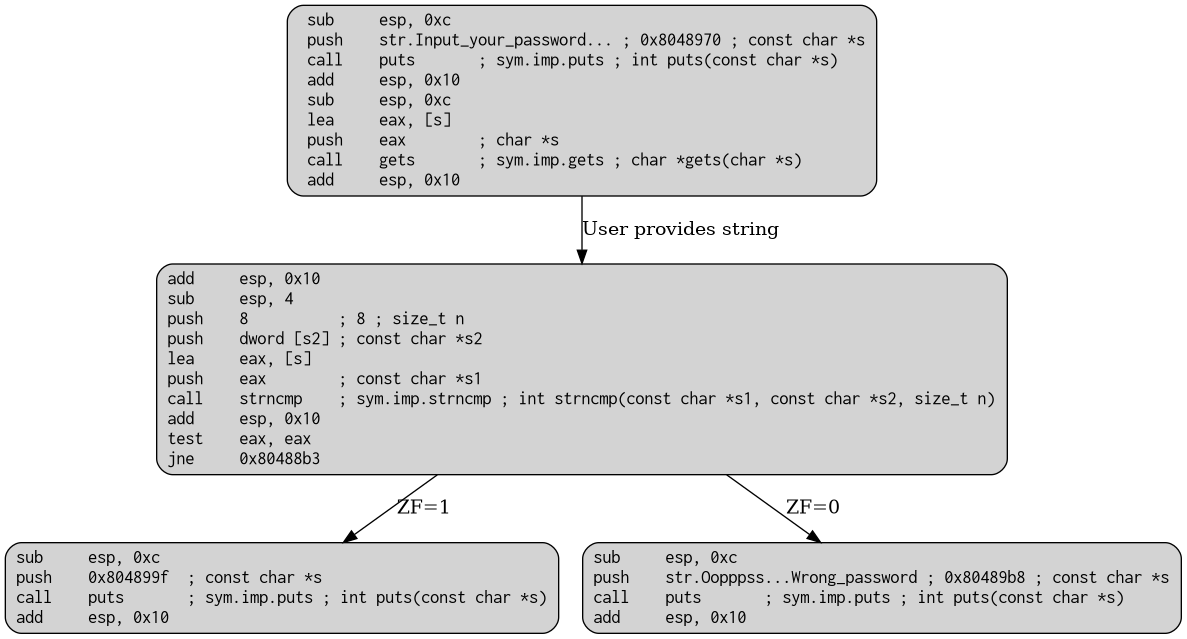
\includegraphics[width=0.99\linewidth]{./graphviz/challenge2.png}
\end{figure}

\section*{Challenge 3}
\subsection*{Goal}
Get the computer to tell me I am amazing.

\subsection*{Steps}

Popping the code into radare2 and looking through it, the code appeared to be looking for a password. I could deduce this because there was a call to a string compare, then a jump if that result was not equal, then a printf with the string I wanted to see. From here I could tell that it was a simple strcmp.
\begin{lstlisting}
    0x080486d4      push    8          ; 8 ; size_t n
    0x080486d6      lea     edx, [s2]
    0x080486d9      push    edx        ; const char *s2
    0x080486da      push    eax        ; const char *s1
    0x080486db      call    strncmp    ; sym.imp.strncmp ; int strncmp(const char *s1, const char *s2, size_t n)
    0x080486e0      add     esp, 0x10
    0x080486e3      test    eax, eax
    0x080486e5      jne     0x80486f7
    0x080486e7      sub     esp, 0xc
    0x080486ea      push    str.You_are_amazing ; 0x80487c4 ; const char *s
\end{lstlisting}

The code pointed to that being the method of conveying the password since there was an \texttt{argc} check earlier in the code. From here I decided that GDB was going to be the quickest line of action. Looking through the assembly, I ascertained the locations of the two strings being used in the comparison.

\begin{lstlisting}
    ; var char **s1 @ ebp-0x2c
    ; var char *s2 @ ebp-0x14 
\end{lstlisting}

\begin{lstlisting}
    Breakpoint 1, 0x080486db in main ()
    (gdb) print (char*)($ebp-0x2c)
    $1 = 0xffffd5dc "\264\326\377\377"
    (gdb) print *(char**)($ebp-0x2c)
    $2 = 0xffffd6b4 "x\330\377\377\262\330\377\377"
    (gdb) print *(char**)($ebp-0x14)
    $3 = 0x33353541 <error: Cannot access memory at address 0x33353541>
    (gdb) print (char*)($ebp-0x14)
    $4 = 0xffffd5f4 "A553Mb1Y"
\end{lstlisting}

I had not fed GDB a valid string as my password (just put some random bytes), so my s1 was going to be garbage. However, the password I needed was stored in plaintext in s2 as "A553Mb1Y", so I was lucky again this time. At this point I knew the password, but had no clue if my password provided was being changed in the code in some capacity (it would be unlikely, but not impossible), but skimming over the assembly this seemed like it was not the case. So tried using the password "A553Mb1Y" as a CLA, and lucky for me it worked.

\subsection*{Answer}
\begin{lstlisting}
    [bentonguess@benton-pc march_27_lab_test]$ ./re_challenge3 A553Mb1Y
    The answer: 1
    Maybe it's this:5
    You are amazing!!
\end{lstlisting}

\subsection*{CFD}
\begin{figure}[H]
    \centering
    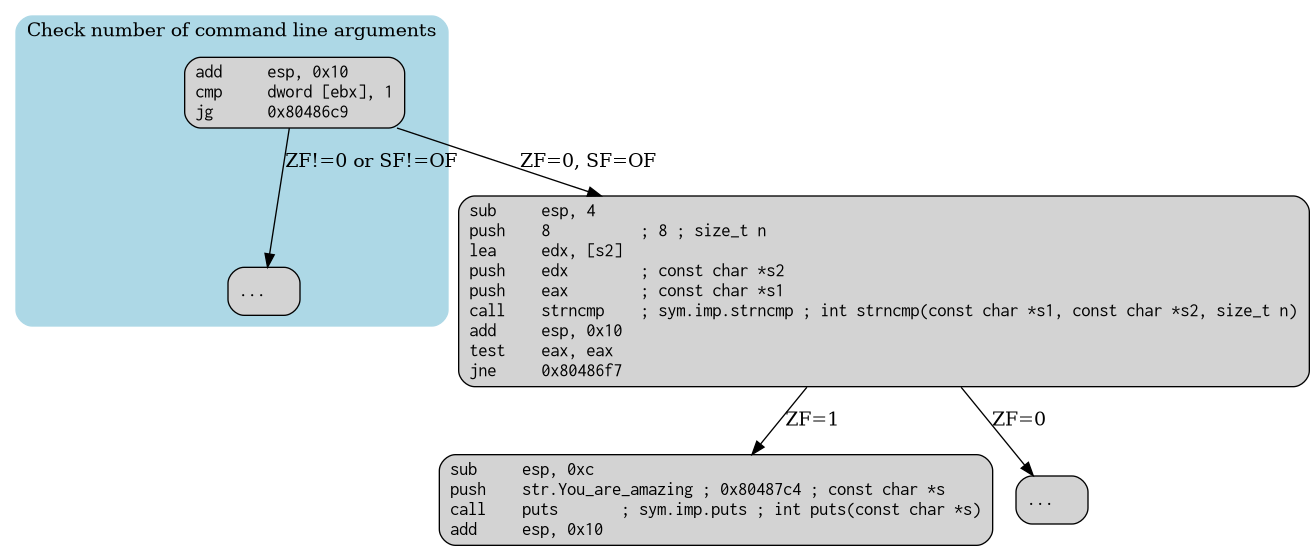
\includegraphics[width=0.99\linewidth]{./graphviz/challenge3.png}
\end{figure}

\end{document}